\chapter{Anexo 1: resultados experimentales}
\label{anexo1}

A continuación se muestran los resultados que hemos obtenido aplicando distintos parámetros a los casos de prueba de los que disponíamos:

\begin{figure}[H]
	\begin{center}
		\centering
		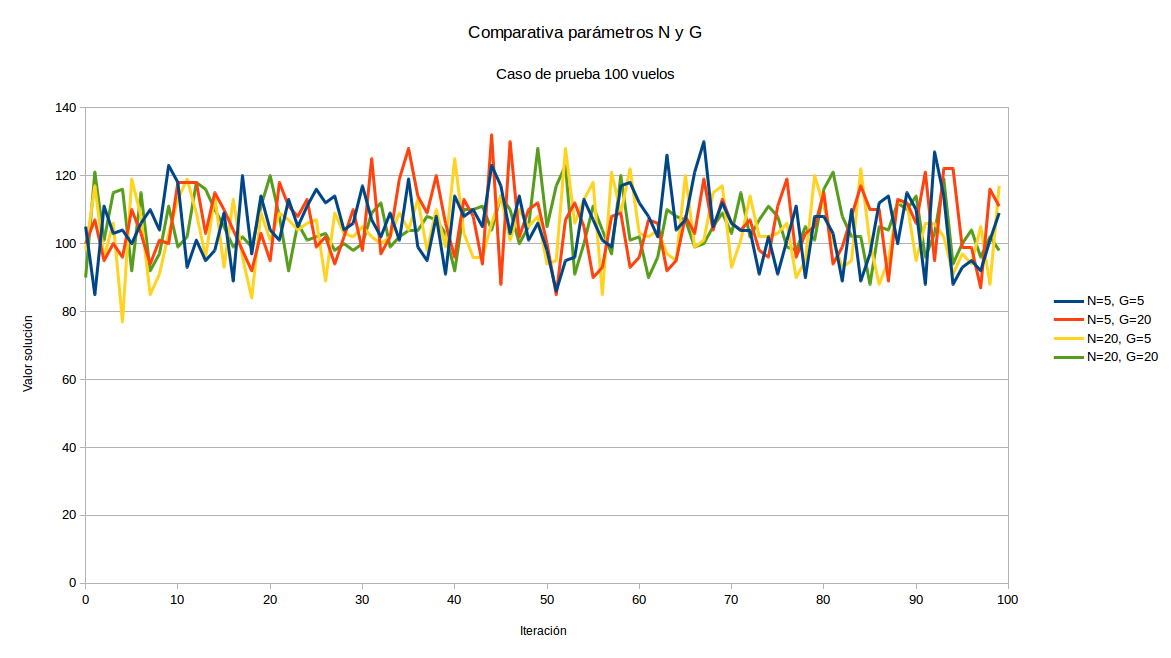
\includegraphics[width=0.8\textwidth]{./imagenes/heuristico/comparativa_parametros_100_vuelos.png}
		\caption{Comparativa de parámetros G y N}
		\label{fig: Comparativa de parámetros G y N}
	\end{center}
\end{figure}


\begin{table}[htbp]
	\centering
	\caption{Comparativa de parámetros $G$ y $N$.}
	\label{fig: comparativa de parámetros $G$ y $N$.}
	\begin{tabular}{|c|c|c|c|}
		\hline
		& \textbf{Problema 1
			100 vuelos} & \textbf{Problema 2
			100 vuelos} & \textbf{Problema 3
			100 vuelos} \\ \hline
		\textbf{N=2, G=10} & \% éxito: 64 & \% éxito: 94 &  \\ \hline
		\textbf{N=2, G=30} & \% éxito: 65 & \% éxito: 95 &  \\ \hline
		\textbf{N=2, G=50} &  &  &  \\ \hline
		\textbf{N=5, G=10} &  &  &  \\ \hline
		\textbf{N=5, G=30} &  &  &  \\ \hline
		\textbf{N=5, G=50} &  &  &  \\ \hline
		\textbf{N=10, G=10} &  &  &  \\ \hline
		\textbf{N=10, G=30} &  &  &  \\ \hline
		\textbf{N=10, G=50} &  &  &  \\ \hline
	\end{tabular}
	
\end{table}


A continuacinó se muestran los resultados obtenidos



\section{Base de datos 1}
\subsection{20 vuelos}
\textcolor{red}{Sobre el 90\%-100\%}
\subsection{100 vuelos}
\textcolor{red}{Sobre el 60\%-70\%}
\subsection{812 vuelos}
\textcolor{red}{SIN PROBAR}

\section{Base de datos 2}
\subsection{20 vuelos}
\textcolor{red}{Sobre el 95\%-100\%}
\subsection{100 vuelos}
\textcolor{red}{Sobre el 90\%}
\subsection{3196 vuelos}
\textcolor{red}{SIN PROBAR}

\section{Base de datos 3}
\subsection{20 vuelos}
\textcolor{red}{Sobre el 95\%-100\%}
\subsection{100 vuelos}
\textcolor{red}{Sobre el 80\%}
\subsection{6475 vuelos}
\textcolor{red}{SIN PROBAR}
